\chapter{Implementation}

This chapter will cover the actual implementation of the project. The whole process of implementation was split into two parts: creation of the MPI Layer and clustering implementation within the Mapper class.

\section{MPI Layer}

The MPI Layer, as mentioned before, operates, based on the two main entities - \textbf{MasterSimulation} and \textbf{WorkerSimulation} classes.

\emph{MasterSimulation} is responsible for clustering and separation of the user input, distribution of this information to the corresponding workers and synchronisation of workers during simulation timesteps. It is the core class of the simulation, as it receives original network parameters, specified by the user.

\emph{WorkerSimulation} (sometimes regarded as nodes) is running the simulation and communicates with Master, to receive user-input information (initialisation parameters), and with other Workers during simulation. This is an auxiliary class, that is fully responsible for the local NeMo simulation running on its cluster.

\subsection{Basic Distributed Platform}

The construction of the basic platform focused on establishing the communication channel between the master simulation and the worker ones. This meant MPI initialisation on both sides, followed by an exchange messages with commonly known communication tags.

The earliest version of the distributed system, that implemented the first design step of building a distributed simulation, consisted of a master, sending out one integer (in this case it was number of neurons to be simulated), that was received by all workers. Once they received this message, self-initialisation of all parameters of the simulation followed, with consequent asynchronous completion after a set number of steps.

\subsubsection{Initial parameters distribution}

Having this initial setup ready, implementation of the second step of distributed version creation followed.
The master simulation, after having both Configuration and Network passed to it, did a basic division of the neurons per worker - distributed those uniformly (until the Mapper is fully implemented):
\begin{equation}N_{per\ worker} = \frac{N_{neurons}}{N_{workers}}\end{equation}
The translation of global id to a local one implemented within mapper at that stage is also simple:
\begin{equation}ID_{global} = ID_{local} + (Rank_{worker}-1)*N_{per\ worker}\end{equation}

\begin{figure}[h]
\begin{center}
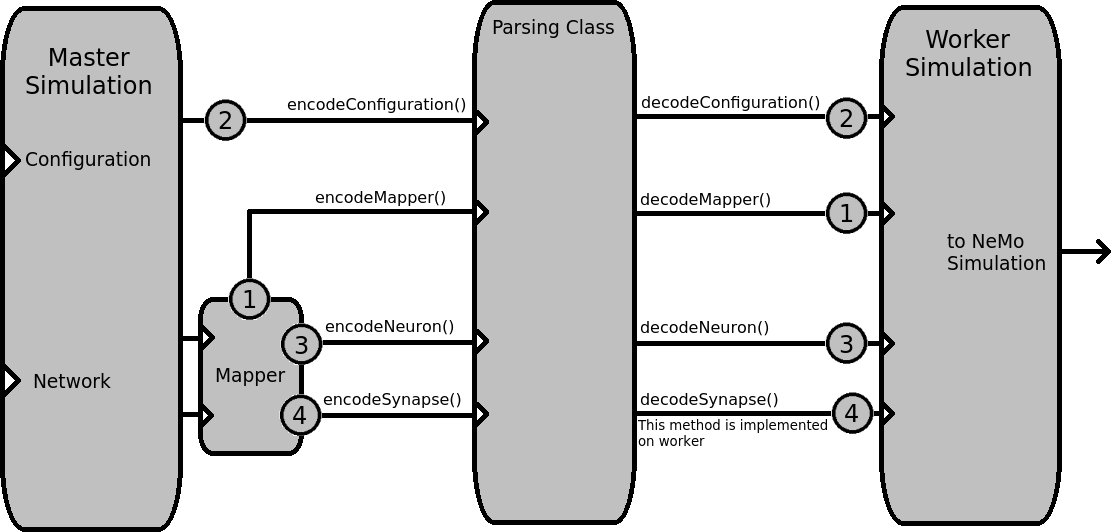
\includegraphics[scale = 0.5]{images/distribution.png}
\end{center}
\caption{Parameters distribution}
\end{figure}

Once the worker set of parameters needed for initialisation was finalised, those need to be encoded and sent out to the workers. This is done through a set of parsing methods - a pair encode-decode for each type of the data. If the data sent is heterogeneous, i.e. more than one primitive datatype is present, the information is encoded into a string of values.

Parsing class was added for the encoding and decoding capabilities - it is accessible by both Master and Worker classes. It provides set of methods for encoding and parsing messages for further use during MPI calls.

The whole distribution stage can be split into 4 distinct steps:

\begin{enumerate}
\item{\textbf{Mapper distribution}}

Mapper has to be encoded with all information present inside - all workers must have the same mapping to ensure correctness of later communication. The data sent is split into a number of strings corresponding to the number of workers and broadcasted for the consequent reconstruction on the sub-simulation.

\item{\textbf{Configuration distribution}}

Configuration is encoded into a string that is also broadcasted to all workers. The information passed does not change, therefore, there is no need to iterate through each master-worker channel.

\item{\textbf{Neuron distribution}}

Once the mapping is set up, the neurons are distributed according to it. Firstly, the worker receives the number of neurons, and then MPI receive method is looped to gather neuronal data. Every string received is decoded, the global index is mapped locally, and, once it is done, a new neuron with this set of parameters is added to the local network.

\item{\textbf{Synapse distribution}}

The last part of the distribution stage, synaptic distribution, is also the most complex - the internal (both source and target are on the same node) synapses are sent as strings to the corresponding worker, whereas external ones need indication for the external target or source. This is done through assigning a negative value to them:
\begin{equation}Value_{external} = -(Value_{internal}+1)\end{equation}

Worker simulations have two data structures for storing incoming and outgoing synapses. The latter is built simply as an array of pairs - local id of a neuron and a vector of targets. The former, however, needs to store the synapse data - local target, weight, delay, plasticity - so it is structured as a vector of vectors of structs. These two are populated as the worker receives and decodes the synaptic data for external synapses.

Note, that even though the external synaptic structure was implemented, it is not put to use at this stage, as there is no spike delivery integrated between sub-simulations within the system at this point.
\end{enumerate}

Once all parameters are received, workers set up their simulations and notify master when it is done. When master receives confirmation from all workers, the simulation may commence, through broadcasting the step signal across the network. 

\subsection{Communication Channels Integration}

At this point the system has a fully operational master-worker distribution channel. Next step is implementation of an inter-worker communication channel used for spike delivery.

First of all, the sources need to be identified, to acquire knowledge of the corresponding targets and their worker location. As given by the NeMo architecture, the simulation step function returns IDs of the neurons fired during this simulation step. These are then used to derive any outgoing spikes, i.e. going through external synapses. The worker step function is done in similar way to the original NeMo implementation, it could be split into three sub-steps\cite{AndreasK.Fidjeland2009}:

\begin{enumerate}
\item {\textbf{Enqueuing Spikes (Prefire)}} 

This is a stage during which the data about incoming currents is collected and passed to the fire function.
Within MPI Simulation, function $enqueueIncomingSpikes()$ provides this functionality, by taking the incoming current data and passing it to the NeMo simulation $step()$ function.

\item {\textbf{Local Simulation Step (Fire)}}

This function determines which neurons have fired by updating the neuron values based on the data collected during prefire step. Original NeMo simulation $step()$ function is used as \emph{Fire} stage returning the vector of fired neurons. The fired neurons are passed to the postfire function.

\item {\textbf{Distributing Spikes (Postire)}}

The final stage of the simulation step, during which the spikes are distributed across the network. Local distribution is done within NeMo step, external is done through series of MPI calls by Worker simulations.
\end{enumerate}

Once a Worker has finished its step, it sends notification to the Master, who, after receiving confirmation from all Workers, advances the global simulation one step further.

After finalisation of overall communication structure, the external delivery design needs to be specified. In the following sections the spike delivery system is given in details.

\subsubsection{Spike Enqueuing}

In order to provide the capacity of storing the incoming spikes, WorkerSimulation class has two data structure for storing those: dequeuing $incoming\_queue$ and priority $delay\_queue$.

The purpose of $incoming\_queue$ is to collect global IDs of all neurons, that have a target on this node. It is populated during the later distribution step.

The $delay\_queue$ is created to store the spikes depending on their delay values. Delay represents number of simulation steps that need to commence before this spike reaches the target node.

\begin{figure}[h]
\begin{center}
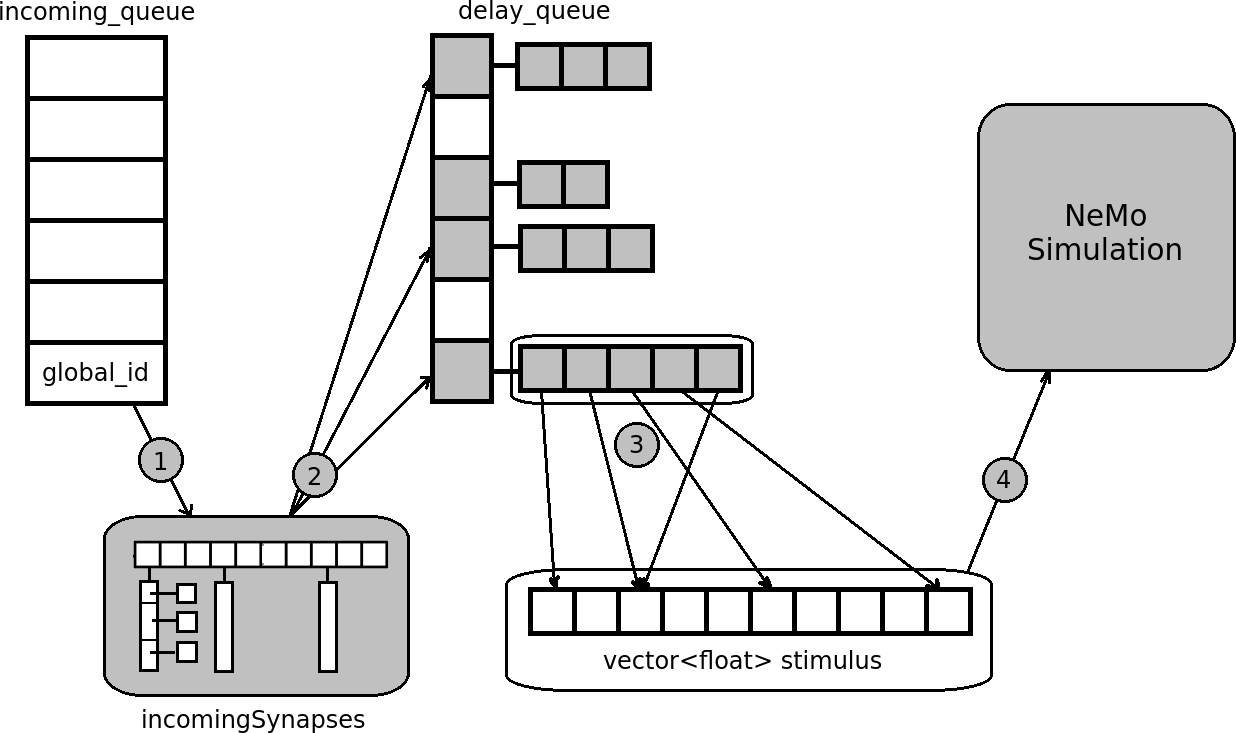
\includegraphics[scale = 0.5]{images/spike_enqueuing_scheme.png}
\end{center}
\caption{Representation of spike enqueuing}
\end{figure}

Taking this into account, $enqueueIncomingSpikes()$ function can be split into two steps:

During first step, it continously dequeues $incoming\_queue$ (1), while it is not empty, looks up the targets connected to this source in Worker's $incomingSynapses$ structure, and puts them into $delay\_queue$ depending on their delays (2). 

The second step commences, after the delay sorting has been resolved. A vector of floats (incoming currents) $stimulus$ is initialised with size corresponding to the number of neurons on the node and values set to 0.0. The head of the delay queue (delay = 1) is poped and iterated through (3). Each entry consists 2 values: target and weight. Using those, the current vector is updated: for each target a synapse weight is added to its current value (4).

The resulting vector is then passed to the local NeMo simulation $step(stimulus)$ function.

\subsubsection{Spike Distribution}

The simulation step returns a vector $fired$ of local neuron IDs, indicating the neurons that have fired. After taking this vector as a parameter, $distributeOutgoingSpikes(fired)$ performs external distribution of spikes.

\begin{figure}[h]
\begin{center}
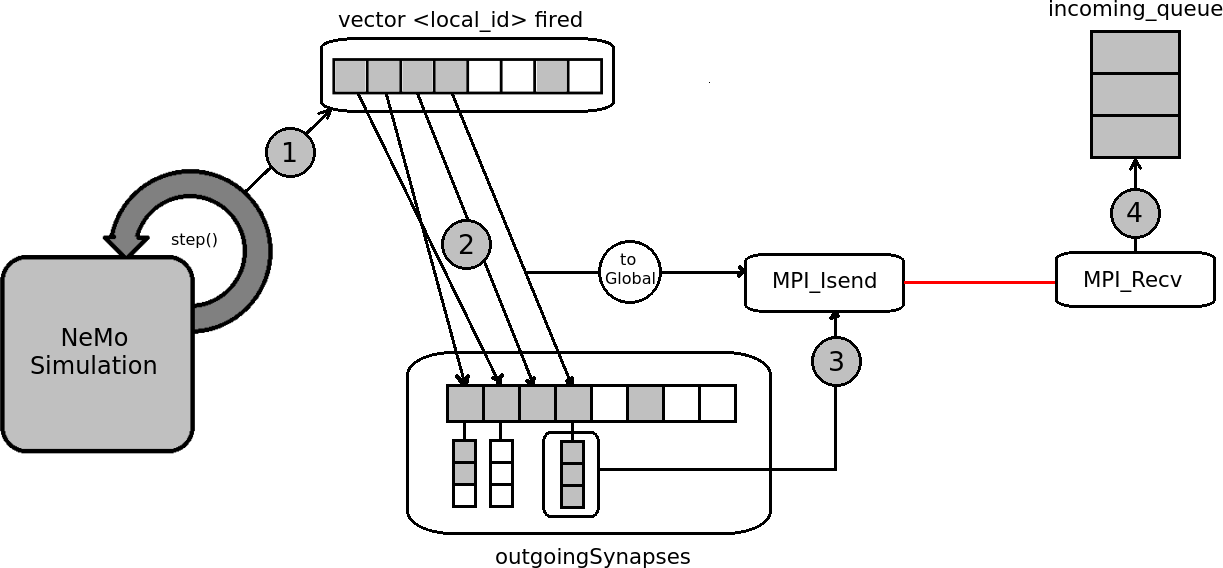
\includegraphics[scale = 0.5]{images/spike_distribution_scheme.png}
\end{center}
\caption{Representation of spike distribution}
\end{figure}

This function can also be split into two steps:

First step: the vector of fired neurons (1) is iterated through, IDs are looked up in the $outgoingSynapses$ structure. As each ID has a vector of corresponding target nodes (2), this vector is iterated through (3), and a non-blocking MPI message with the global ID of a neuron is sent to the target. After the distribution is finalised, an ending message is sent to all workers.

Second step: after all non-blocking messages have been sent, function initiates a loop that enqueues (4) all incoming IDs into the $incoming\_queue$. This loop only terminates after receiving the ending messages from all other workers.

After finishing these two steps, the function returns, leading to the end of the distributed simulation step on this worker.

\section{Clustering}

Clustering implementation is dependent on the algorithm introduced by Mark Newman in 2006. This section will provide the mathematical overview of this algorithm and its implementation within Mapper class.

\subsection{Newman's Algorithm}

Major part of Newman's research concentrates on finding communities in the network structures\cite{NewmanComm}. \emph{Community structure} is a feature of a graph that shows the gathering of vertices into groups with high connectivity. This feature is best described by modularity, the measure of modular division of a particular network into subnets with high edge density.

Formula for modularity is:
\begin{equation}\end{equation}

Newman's algorithm ("Method of Optimal Modularity"\cite{Newman2006}) is a way of determining the natural division of graph's vertices into several non-overlapping communities, based on the modularity measure. 

\begin{enumerate}
\item{Create an adjancency matrix of the network}
\item{Matrix Q is created with the same dimensions as the adjacency one. The values in Q matrix are set through using equation: 
\begin{equation}Q[i][j] = A[i][j] - \frac{k_{i}k_{j}}{2m}\end{equation}
where $k_{i}$ and $k_{j}$ degrees of corresponding neurons, and m is the total number of synapses}
\item{For the resulting Q matrix the dominating eigen vector has to be generated - this is done through the use of power-iteration algorithm}
\item{The values of eigenvector correspond to the split of this network into two parts - any further division is done by applying this algorithm again}
\end{enumerate}

\subsection{Mapper integration}

\begin{figure}[h]
\begin{center}

\includegraphics[scale = 0.5]{images/placeholder.png}
\end{center}
\caption{Clustering function}
\end{figure}

\section{Alternative Solutions}

\begin{itemize}
\item{Use of Boost libraries}

Use of Boost libraries was not possible early in the project due to the build fails - after a certain checkpoint it was already inefficient to regurgitate through the whole code to recreate the capabilities.
\end{itemize}
